%\iffalse
\let\negmedspace\undefined
\let\negthickspace\undefined
\documentclass[journal,12pt,twocolumn]{IEEEtran}
\usepackage{cite}
\usepackage{amsmath,amssymb,amsfonts,amsthm}
\usepackage{algorithmic}
\usepackage{graphicx}
\usepackage{textcomp}
\usepackage{xcolor}
\usepackage{txfonts}
\usepackage{listings}
\usepackage{enumitem}
\usepackage{mathtools}
\usepackage{gensymb}
\usepackage{comment}
\usepackage[breaklinks=true]{hyperref}
\usepackage{tkz-euclide} 
\usepackage{listings}
\usepackage{gvv}                            \usepackage{tikz}
\usepackage{circuitikz}
\def\inputGnumericTable{}                                
\usepackage[latin1]{inputenc}                            
\usepackage{color}                                       
\usepackage{array}                                       
\usepackage{longtable}                                   
\usepackage{calc}                              
\usepackage{tikz}
\usepackage{multirow}                                    
\usepackage{hhline}                                      
\usepackage{ifthen}                            
\usepackage{caption}
\usepackage{lscape}
\usepackage{amsmath}
\newtheorem{theorem}{Theorem}[section]
\newtheorem{problem}{Problem}
\newtheorem{proposition}{Proposition}[section]
\newtheorem{lemma}{Lemma}[section]
\newtheorem{corollary}[theorem]{Corollary}
\newtheorem{example}{Example}[section]
\newtheorem{definition}[problem]{Definition}
\newcommand{\BEQA}{\begin{eqnarray}}
\newcommand{\EEQA}{\end{eqnarray}}
\newcommand{\define}{\stackrel{\triangle}{=}}
\theoremstyle{remark}
\newtheorem{rem}{Remark}

\begin{document}

\bibliographystyle{IEEEtran}
\vspace{3cm}

\title{GATE 2022 IN.53}
\author{EE23BTECH11010 - VENKATESH BANDAWAR$^{*}$% <-this % stops a space
}
\maketitle
\newpage
\bigskip
\textbf{Question:} In a unity-gain feedback control system, the plant
$P(s) = \frac{0.001}{s\brak{2s+1}\brak{0.01s+1}}$
is controlled by a lag compensator
$C(s) = \frac{s+10}{s+0.1}$
The slope (in dB/decade) of the asymptotic Bode magnitude plot of the loop gain
at $\omega= 3 $rad/s is \_\_\_\_\_\_\_\_ (in integer)
\hfill(GATE 2022 IN)\\
\solution
\begin{table}[!h]
    \centering
    \begin{tabular}{|c|c|c|}
\hline
    Parameter & Description & Value\\
    \hline
    $P(s)$ & Plant Transfer Function & $\frac{0.001}{s\brak{\frac{s}{0.5}+1}\brak{\frac{s}{100}+1}}$\\
    \hline
    $C(s)$ & Lag Compensator  & $\frac{100\brak{\frac{s}{10}+1}}{\frac{s}{0.1}+1}$\\
    \hline
    $T(s)$ & Loop gain  & $P(s) C(s)$ \\
    \hline
    $\omega$ & Angular Frequency & 3rad/s \\
    \hline
\end{tabular}

    \caption{Given Parameters list}
    \label{tab:Given Parameters list.gate2022.IN.53}
\end{table}

let $j\omega = s$\\
The slope of the asymptotic Bode magnitude plot of the loop gain= $20\log_{10}\abs{L\brak{j\omega}}$
\begin{align}
    \omega &= 3\\
    L\brak{j\omega} &= \frac{0.001\brak{3j+10}}{3j\brak{6j+1}\brak{0.03j+1}\brak{3j+0.1}}\\
    slope &\approx 20 \log_{10}\frac{0.001\times \sqrt{109}}{3\times \sqrt{37} \times 1 \times 3}\\
    &\approx -74  dB/decade
\end{align}
\begin{figure}[!h]
    \centering
    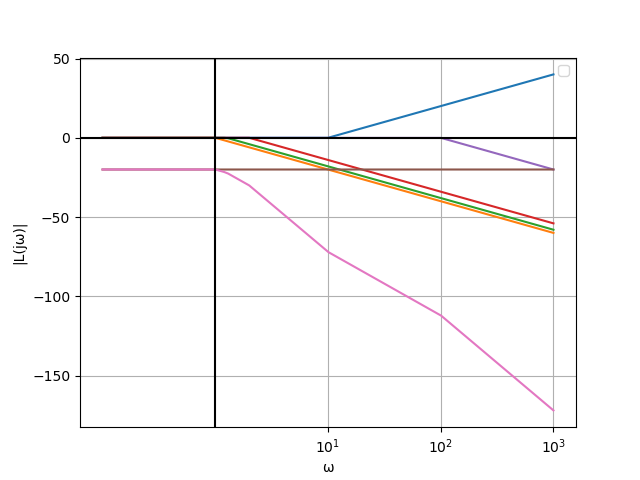
\includegraphics[width=\columnwidth]{figs/bode_mag_plot.png}
    \caption{Bode magnitude plot of loop gain}
\end{figure}

\end{document}
